\documentclass[11pt]{article}
\RequirePackage{fullpage}
\RequirePackage[font=small,labelfont=bf]{caption}
\RequirePackage{amsmath,amssymb,amsthm}
\RequirePackage{mathtools}
\RequirePackage{graphicx}
\RequirePackage[normalem]{ulem}
\RequirePackage[hidelinks]{hyperref}
\RequirePackage{wrapfig}
\RequirePackage{subcaption}
\RequirePackage{authblk}
\RequirePackage{bm}
\RequirePackage{bbm}
\RequirePackage{tikz}
\RequirePackage{xr}

% line numbers:
\RequirePackage{lineno}
%\modulolinenumbers[5]
\renewcommand\linenumberfont{\normalfont\tiny\sffamily\color{black}}

% spacing
\RequirePackage{setspace}
%\doublespacing
 
% \RequirePackage[osf]{mathpazo}
\RequirePackage[bibstyle=authoryear,citestyle=authoryear-comp,
                date=year,
                maxbibnames=99,maxnames=99,maxcitenames=2,
                backend=biber,uniquelist=false,uniquename=false,
                % style=apa,
                dashed=false,
                sorting=nyt,
                hyperref=true]{biblatex}
\RequirePackage[colorinlistoftodos]{todonotes}  %disable
\RequirePackage{color}
\RequirePackage{nicefrac}

\AtEveryBibitem{%
  \clearlist{language}%
}
\renewbibmacro{in:}{}

\newcommand{\gc}[1]{{\it \color{red} #1 } }
\newcommand{\vb}[1]{{\it \color{blue} #1}}
\newcommand{\vbout}[1]{{\it \color{blue} \sout{#1}}}

% a /nonumber you can turn on/off
\newcommand{\nnn}{\nonumber}
%\newcommand{\nnn}{}

\newcommand{\beginsupplement}{%
        \setcounter{table}{0}
        \renewcommand{\thetable}{S\arabic{table}}%
        \setcounter{figure}{0}
        \renewcommand{\thefigure}{S\arabic{figure}}%
     }


\newcommand{\graham}[1]{\todo[size=\scriptsize, color=red!50]{#1}}
\newcommand{\vince}[1]{\todo[size=\scriptsize, color=blue!50]{#1}}

\renewcommand{\P}{\mathbb{P}}
\newcommand{\E}{\mathbb{E}}
\newcommand{\V}{\text{V}}
\newcommand{\cf}{\emph{cf.} }
\DeclareMathOperator{\var}{Var}
\DeclareMathOperator{\cov}{Cov}
\DeclareMathOperator{\flt}{\mathrm{flat}}
\DeclareMathOperator{\T}{{\mathrm{T}}}
\newcommand{\vect}[1]{\mathbf{#1}}
\newcommand{\nssh}{SSH_n}

\newcommand{\chapquote}[2]{\begin{quotation} \textit{#1} \end{quotation} \begin{flushright} - #2\end{flushright} }

\addbibresource{biblio.bib}

\externaldocument{supp}



% TODO
% - divide through the temp block supp. figure by combinatorics
% - mention PCA



\title{Estimating the genome-wide contribution of selection to temporal allele frequency change}


% A long-standing problem in evolutionary biology is to understand the processes
% that shape the genetic composition of populations. In a population without
% migration, the two processes that change allele frequencies are selection,
% which increases beneficial alleles and removes deleterious ones, and genetic
% drift which randomly changes frequencies as some parents contribute more or
% less alleles to the next generation. Previous efforts to disentangle these
% processes have used genomic samples from a single timepoint and models of how
% selection affects neighboring sites (linked selection). Here, we use genomic
% data taken through time to quantify the contributions of selection and drift to
% genome-wide frequency changes. We show selection acts over short timescales in
% three evolve-and-resequence studies and has a sizeable genome-wide impact.

\author[$\ast$,$\dag$,$1$]{Vince Buffalo}
\author[$\dag$]{Graham Coop}
\affil[$\ast$]{\footnotesize Population Biology Graduate Group}
\affil[$\dag$]{\footnotesize Center for Population Biology, Department of Evolution and Ecology, University of California, Davis, CA 95616}
\affil[$1$]{\footnotesize Email for correspondence: \href{mailto:vsbuffalo@ucdavis.edu}{vsbuffalo@ucdavis.edu}}

\begin{document}
\maketitle

\linenumbers

\begin{abstract}

  Rapid phenotypic adaptation is often observed in natural populations and
  selection experiments. However, detecting the genome-wide impact of this
  selection is difficult, since adaptation often proceeds from standing
  variation and selection on polygenic traits, both of which may leave faint
  genomic signals indistinguishable from a noisy background of genetic drift.
  One promising signal comes from the genome-wide covariance between allele
  frequency changes observable from temporal genomic data, e.g.
  evolve-and-resequence studies. These temporal covariances reflect how
  heritable fitness variation in the population leads changes in allele
  frequencies at one timepoint to be predictive of the changes at later
  timepoints, as alleles are indirectly selected due to remaining associations
  with selected alleles. Since genetic drift does not lead to temporal
  covariance, we can use these covariances to estimate what fraction of the
  variation in allele frequency change through time is driven by linked
  selection. Here, we reanalyze three selection experiments to quantify the
  effects of linked selection over short timescales using covariance among
  time-points and across replicates. We estimate that at least 17\% to 37\% of
  allele frequency change is driven by selection in these experiments. Against
  this background of positive genome-wide temporal covariances we also identify
  signals of negative temporal covariance corresponding to reversals in the
  direction of selection for a reasonable proportion of loci over the time
  course of a selection experiment. Overall, we find that in the three studies
  we analyzed, linked selection has a large impact on short-term allele
  frequency dynamics that is readily distinguishable from genetic drift.

\end{abstract}

\subsubsection*{Significant Statement}

A long-standing problem in evolutionary biology is to understand the processes
that shape the genetic composition of populations. In a population without
migration, the two processes that change allele frequencies are selection,
which increases beneficial alleles and removes deleterious ones, and genetic
drift which randomly changes frequencies as some parents contribute more or
less alleles to the next generation. Previous efforts to disentangle these
processes have used genomic samples from a single timepoint and models of how
selection affects neighboring sites (linked selection). Here, we use genomic
data taken through time to quantify the contributions of selection and drift to
genome-wide frequency changes. We show selection acts over short timescales in
three evolve-and-resequence studies and has a sizeable genome-wide impact.



\section{Introduction}

A long-standing problem in evolutionary genetics is quantifying the roles of
genetic drift and selection in shaping genome-wide allele frequency changes.
Selection can affect allele frequencies, both directly and indirectly, with the
indirect effect coming from the action of selection on correlated loci
elsewhere in genome, e.g. linked selection (\cite{Maynard_Smith1974-zr},
\cite{Charlesworth1993-gb,Nordborg1996-nq}; see \cite{Barton2000-zg} for a
review). Previous work has mostly focused on teasing apart the impacts of drift
and selection on genome-wide diversity using population samples from a single
contemporary timepoint, often by modeling the correlation between regional
recombination rate, gene density, and diversity created in the presence of
linked selection \parencite{Cutter2013-ba,Sella2009-nx}. This approach has
shown linked selection has a major role in shaping patterns of genome-wide
diversity across the genomes of a range of sexual species
\parencite{Macpherson2007-qt,Andolfatto2007-uy,Begun2007-bg,Beissinger2016-cm,Sattath2011-dr,Williamson2014-oy,Andersen2012-bj,Cutter2010-gi,Elyashiv2016-vt},
and has allowed us to quantify the relative influence of positive selection
(hitchhiking) and negative selection (background selection;
\cite{Nordborg2005-dc,McVicker2009-ax,Andolfatto2007-uy,Macpherson2007-qt,Hernandez2011-gs,Elyashiv2016-vt}).
However, we lack an understanding of both how linked selection acts over short
time intervals and its full impact on genome-wide allele frequency changes.

There are numerous examples of rapid phenotypic adaptation
\parencite{Grant2011-wk,Grant2006-hj,Reznick1997-mh,Franks2007-dr} and rapid,
selection-driven genomic evolution in asexual populations
\parencite{Good2017-om,Bennett1990-bc,Baym2016-kh}.  Yet the polygenic nature
of fitness makes detecting the impact of selection on genome-wide variation
over short timescales in sexual populations remarkably difficult
\parencite{Latta1998-me, Pritchard2010-tk,Kemper2014-bx}. This is because the
effect of selection on a polygenic trait (such as fitness) is distributed
across numerous loci. This can lead to subtle allele frequency shifts on
standing variation that are difficult to distinguish from background levels of
genetic drift and sampling variance. Increasingly, genomic experimental
evolution studies with multiple timepoints, and in some cases multiple
replicate populations, are being used to detect large-effect selected loci
\parencite{Turner2011-sx,Turner2012-bm} and differentiate modes of selection
\parencite{Burke2010-tz,Barghi2019-qy,Therkildsen2019-zy}.  In addition these
temporal-genomic studies have begun in wild populations, some with the goal of
finding variants that exhibit frequency changes consistent with fluctuating
selection \parencite{Bergland2014-ij,Machado2018-cs}. In a previous paper, we
proposed that one useful signal for understanding the genome-wide impact of
polygenic linked selection detectable from temporal genomic data is the
temporal autocovariance (i.e. covariance between two timepoints) in allele
frequency changes \parencite{Buffalo2019-io}.  These covariances are created
when the loci that underly heritable fitness variation perturb the frequencies
of linked alleles; in contrast, when genetic drift acts alone in a closed
population, these covariances are expected to be zero for neutral alleles.
Mathematically, temporal covariances are useful because it is natural to
decompose the total variance in allele frequency change across a time interval
into the variances and covariances in allele frequency change between
generations.  Furthermore, biologically, these covariances reflect the extent
to which allele frequency changes in one generation predict changes in another
due to a shared selection pressures and associations to selected loci.

Here, we provide the first empirical analyses to quantify the impact of linked
selection acting over short timescales (tens of generations) across two evolve
and re-sequence studies \parencite{Barghi2019-qy,Kelly2019-dc}, and an
artificial selection experiment \parencite{Castro2019-uk}. These sequencing
selection experiments have started to uncover selected loci contributing to the
adaptive response; however it is as yet far from clear how much of the allele
frequency genome-wide is driven by selection or genetic drift. We repeatedly
find a signal of temporal covariance, consistent with linked selection acting
to significantly perturb genome-wide allele frequency changes across the genome
in a manner that other approaches would not be able differentiate from genetic
drift. We estimate a lower bound of the fraction of variance in allele
frequency change caused by selection, as well as the correlation between allele
frequency changes between replicate populations caused by convergent selection
pressures. Overall, we demonstrate that linked selection has a powerful role in
shaping genome-wide allele frequency changes over very short timescales.

\section{Results}

\begin{table}
  \centering
  \footnotesize
  \centering
  \begin{tabular}{l c c c c c c}
    \textbf{Study} & \textbf{Species} & \textbf{Selection} & \textbf{Replicates} & \textbf{Pop. Size}$^{\dagger}$ & \textbf{Gens.} & \textbf{Timepoints} \\ 
  \hline
    \textcite{Kelly2019-dc}  & \emph{D. simulans} & lab adaptation & 3 & $\sim$1100 & 14 & 2 \\ \hline
    \textcite{Barghi2019-qy} & \emph{D. simulans} & lab adaptation & 10 & $\sim$1000 & 60 & 7 \\ \hline
    \textcite{Castro2019-uk} & \emph{M. musculus} & \begin{tabular}{c}tibiae length\\control\end{tabular} & \begin{tabular}{c}2\\1\end{tabular} &\begin{tabular}{c}32\\28\end{tabular}  & 17 & 2 \\
 \hline
  \end{tabular}
  \caption{A summary of the main selection studies we
    analyzed. $^{\dagger}$Approximate census population size
      during experiment.} 
      \label{table:study_summary} 
\end{table}

We first analyzed \textcite{Barghi2019-qy}, an evolve-and-resequence study with
ten replicate populations exposed to a high temperature lab environment and
evolved for 60 generations, and sequenced every ten generations. Using the
seven timepoints and ten replicate populations, we estimated the genome-wide $6
\times 6$ temporal covariance matrix $\mathbf{Q}$ for each of the ten
replicates. Each row of these matrices represent the temporal covariance
$\cov(\Delta_{_{10}} p_s, \Delta_{_{10}} p_t)$, between the allele frequency
change (in ten-generation intervals, denoted $\Delta_{_{10}} p_t$) of some
initial reference generation $s$ (the row of the matrix), and some later
timepoint $t$ (the column of the matrix). We corrected these matrices for
biases created due to sampling noise, and normalized the entries for
heterozygosity (see Supplementary Materials Sections
\ref{supp:ind-depth-var-corr} and \ref{supp:matrix-correction}). These
covariances are expected to be zero when only drift is acting, as only
heritable variation for fitness can create covariance between allele frequency
changes in a closed population \parencite{Buffalo2019-io}.  Averaging across
the ten replicate temporal covariances matrices, we find temporal covariances
that are statistically significant (95\% block bootstraps CIs do not contain
zero), consistent with linked selection perturbing genome-wide allele frequency
changes over very short time periods. The covariances between all adjacent time
intervals are positive and then decay towards zero as we look at more distant
time intervals (Figure \ref{fig:figure-1} A), as expected when directional
selection affects linked variants' frequency trajectories until ultimately
linkage disequilibrium and the associated additive genetic variance for fitness
decays (which could occur as a population reaches a new optimum)
\parencite{Buffalo2019-io}. The temporal covariances per replicate are noisier
but this general pattern holds; see Supplementary Figure
\ref{suppfig:barghi-cov-panels}. 

Since our covariances are averages over loci, the covariance estimate could be
strongly affected by a few outlier regions. To test whether large outlier
regions drive the genome-wide signal we see in the \textcite{Barghi2019-qy}
data, we calculate the covariances in 100kb windows along the genome (we refer
to these as windowed covariances throughout) and take the median windowed
covariance, and trimmed-mean windowed covariance, as a measure of the
genome-wide covariance robust to large-effect loci. These robust estimates
(Supplementary Table \ref{supp:table-trimmed-mean} and Supplementary Figure
\ref{suppfig:barghi-trimmed-mean}) confirm the patterns we see using the mean
covariance, confirming that genomic temporal covariances are non-zero due to
the impact of selection acting across many genomic regions. 


\begin{figure}[!htb]
  \centering
  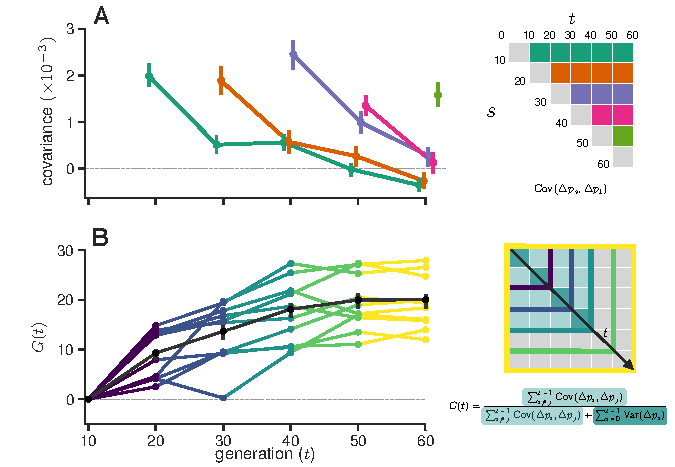
\includegraphics[width=\textwidth]{figure-1-revision.pdf}

  \caption{{\bf A}: Temporal covariance, averaged across all ten replicate
    populations, through time from the \textcite{Barghi2019-qy} study. Each
    line depicts the temporal covariance $\cov(\Delta p_s, \Delta p_t)$ from
    some reference generation $s$ to a later time $t$ which varies along the
    x-axis; each line corresponds to a row of the upper-triangle of the
    temporal covariance matrix with the same color (upper right). The ranges
    around each point are $95\%$ block-bootstrap confidence intervals. {\bf B}: The
    proportion of the total variance in allele frequency change explained by
    linked selection, $G(t)$, as it varies through time $t$ along the x-axis.
    The black line is the $G(t)$ averaged across replicates, with the $95\%$
    block-bootstrap confidence interval. The other lines are the $G(t)$ for
    each individual replicate, with colors indicating what subset of the
    temporal-covariance matrix to the right is being included in the
  calculation of $G(t)$.}

  \label{fig:figure-1}
\end{figure}

While the presence of positive temporal covariances is consistent with
selection affecting allele frequencies over time, this measure is not easily
interpretable. We can calculate a more intuitive measure from the temporal
covariances to quantify the impact of selection on allele frequency change: the
ratio of total covariance in allele frequency change to the total variance in
allele frequency change. We denote the change in allele frequency as $\Delta
p_t = p_{t+1}-p_t$, where $p_t$ is the allele frequency in generation $t$.
Since the total variation in allele frequency change can be partitioned into
variance and covariance components, $\var(p_t - p_0) = \sum_{i=0}^{t-1}
  \var(\Delta p_i) + \sum_{i=0}^{t-1} \sum_{j \ne i}^{t-1} \cov(\Delta p_i,
\Delta p_j)$ (we bias-correct these for sequencing depth), and the
covariances are zero when drift acts alone, this is a lower bound on how much
of the variance in allele frequency change is caused by linked selection
\parencite{Buffalo2019-io}. We call this measure $G(t)$, defined as

\begin{align}
  G(t) = \frac{ \sum_{i=0}^{t-1} \sum_{j \ne i}^{t-1} \cov(\Delta p_i, \Delta p_j)}{\var(p_t - p_0)}
\end{align}
%
which estimates the impact of selection on allele frequency change between
the initial generation $0$ and some later generation $t$, which can be varied
to see how this quantity grows through time. When the sum of the covariances is
positive, this measure can intuitively be understood as the relative fraction
of allele frequency change normally thought of as ``drift" that is actually due
to selection. Additionally, $G(t)$ can be understood as a short-timescale
estimate of the reduction in neutral diversity due to linked selection (or
equivalently the reduction in neutral effective population size needed to
account linked selection, see Supplementary Materials Section
\ref{supp:reduction-approx}). Since \textcite{Barghi2019-qy} experiment is
sequenced every ten generations, the numerator uses the covariances
  estimated between ten-generation blocks of allele frequency change; thus
  the strong, unobservable, covariances between adjacent generations do not
contribute to the numerator of $G(t)$. Had these covariances been measurable
on shorter timescales, their cumulative effect would likely have been higher
yet (see Supplementary Material Sections \ref{supp:barghi-covs} and
\ref{supp:tempblocks} for more details).  Additionally, selection also inflates
the variance in allele frequency change per generation; however, this effect
cannot be easily distinguished from drift. For both these reasons, our measure
$G(t)$ is quite conservative (we demonstrate this through
simulations in Supplementary Material Section \ref{supp:tempblocks}).  Still,
we find a remarkably strong signal. Greater than $20\%$ of total, genome-wide
allele frequency change over 60 generations is the result of selection (Figure
\ref{fig:figure-1} B). This proportion of variance attributable to selection
builds over time in Figure \ref{fig:figure-1}B as the effects of linked
selection are compounded over the generations unlike genetic drift. Our G(t)
starts to plateau to a constant level as the covariances from earlier
generations have decayed and so no longer contribute as strongly (Figure
\ref{fig:figure-1}).

Additionally, we looked for a signal of temporal autocovariance in
\textcite{Bergland2014-ij}, a study that collected \emph{Drosophila
melanogaster} through Spring-Fall season pairs across three years. If there was
a strong  pattern of genome-wide fluctuating selection, we might expect a
pattern of positive covariances between similar seasonal changes, e.g.
Spring-Fall in two adjacent years, and negative covariances between dissimilar
seasonal changes, e.g. Spring-Fall and Fall-Spring in two adjacent years.
However, we find no such signal over years, and in reproducing their original
analysis, we find that their number of statistically significant seasonal SNPs
is not enriched compared to an empirical null distribution created by permuting
seasonal labels; we discuss this in more depth in Supplementary Materials
Section \ref{supp:bergland-reanalysis}.

The replicate design of \textcite{Barghi2019-qy} allows us to quantify another
covariance: the covariance in allele frequency change between replicate
populations experiencing convergent selection pressures. These
between-replicate covariances are created in the same way as temporal
covariances: alleles linked to a particular fitness background are
expected to have allele frequency changes in the same direction if the
selection pressures are similar. Intuitively, where temporal covariances
reflect that alleles associated with heritable fitness backgrounds are
predictive of frequency changes between generations, replicate covariances
reflect that heritable fitness backgrounds common to each replicate predict
(under the same selection pressures) frequency changes between replicates. We
measure this through a statistic similar to a correlation, which we call the
convergent correlation: the ratio of average between-replicate covariance
across all pairs to the average standard deviation across all pairs of
replicates, 


\begin{align}
  \label{eq:conv-corr}
  \mathrm{cor}(\Delta p_s, \Delta p_t) = \frac{\E_{A\ne B} \left( \cov(\Delta p_{s,A}, \Delta p_{t,B}) \right)}{\E_{A\ne B} \left( \sqrt{\var(\Delta p_{s,A}) \var(\Delta p_{t,B})} \right)}
\end{align}
%
where $A$ and $B$ here are two replicate labels, and for the
\textcite{Barghi2019-qy} data, we use $\Delta_{_{10}} p_t$. 

We've calculated the convergent correlation for all rows of the replicate
covariance matrices. Like temporal covariances, we visualize these through time
(Figure \ref{fig:figure-2}A), with each line representing the convergent
correlation from a particular reference generation $s$ as it varies with $t$
(shown on the x-axis). In other words, each of the colored lines corresponds to
the like-colored row of the convergence correlation matrix (upper left in
Figure \ref{fig:figure-2}A). We find these convergent correlation coefficients
are relatively weak, and decay very quickly from an initial value of about 0.1
(95\% block bootstrap confidence intervals $[0.094, 0.11]$) to around 0.01
(95\% CIs [0.0087, 0.015]) within 20 generations. This suggests that while a
substantial fraction of the initial response is shared over the replicates,
this is followed by a rapid decay, a result consistent with the primary finding
of the original \textcite{Barghi2019-qy} study: that alternative loci
contribute to longer term adaptation across the different replicates. 

\begin{figure}[!htb]
  \centering
  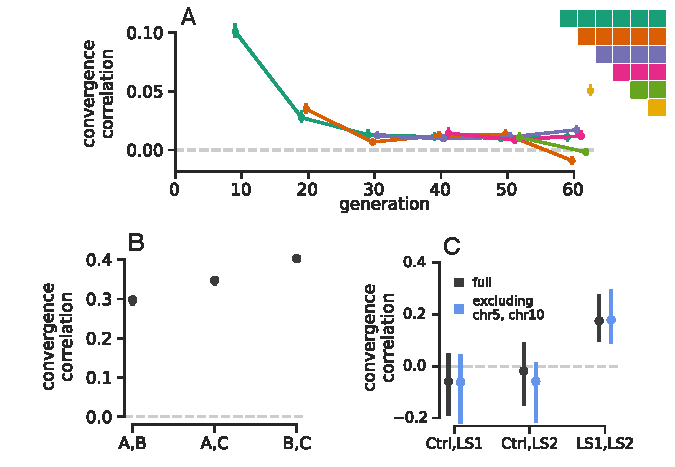
\includegraphics[width=\textwidth]{figure-2-revision.pdf}

  \caption{{\bf A}: The convergence correlations, averaged across
    \textcite{Barghi2019-qy} replicate pairs, through time. Each line
    represents the convergence correlation $\mathrm{cor}(\Delta p_{s}, \Delta
    p_{s})$ from a starting reference generation $s$ to a later time $t$, which
    varies along the x-axis; each line corresponds to a row of the temporal
    convergence correlation matrix depicted to the right (where the
      diagonal elements represent the convergence correlations between the same
      timepoints across replicate populations). We note that convergent
      correlation for the last timepoint is an outlier; we are unsure as to the
      cause of this, e.g. it does not appear to be driven by a single pair of
      replicates. {\bf B}: The convergence correlations between individual
      pairs of replicates in the \textcite{Kelly2019-dc} data (note the
      confidence intervals are plotted, but are small on this y-axis scale).
      {\bf C}:  The convergence correlations between individual pairs of
      replicates in \parencite{Castro2019-uk} data, for the two selection lines
      (LS1 and LS2) and the control (Ctrl); gray CIs are those using the
      complete dataset, blue CIs exclude chromosomes 5 and 10 which harbor the
      two regions \textcite{Castro2019-uk} found to have signals of parallel
      selection between LS1 and LS2. Through simulations, we have found
        that the differences in convergence correlation confidence interval
        widths between these \emph{Drosophila} studies and the Longshanks study
        are due to the differing population sizes.}

  \label{fig:figure-2}
\end{figure}

A benefit of between-replicate covariances is that unlike temporal covariances,
these can be calculated with only two sequenced timepoints and a replicated
study design. This allowed us to assess the impact of linked selection in
driving convergent patterns of allele frequency change across replicate
populations in two other studies. First, we reanalyzed the selection experiment
of \textcite{Kelly2019-dc}, which evolved three replicate wild populations of
\emph{Drosophila simulans} for 14 generations adapting to a novel laboratory
environment. Since each replicate was exposed to the same selection pressure
and share linkage disequilibria common to the original natural founding
population, we expected each of the three replicate populations to have
positive convergence correlations.  We find all three convergent
correlation coefficients between replicate pairs are significant (Figure
\ref{fig:figure-2}B), and average to 0.36 ($95\%$ CI $[0.31, 0.40]$).
Additionally, we can calculate the proportion of the total variance in
allele frequency change from convergent selection pressure, analogous to
our $G(t)$, where the numerator is the convergent covariance and the
denominator is the total variance (see Supplementary Material
\ref{supp:replicate-g}). We find that 37\% of the total variance is due to
shared allele frequency changes caused by selection (95\% CI [29\%, 41\%];
these are similar to the convergence correlation, since the variance is
relatively constant across the replicates.

% 95\% CIs, [0.00635, 0.00860], [0.00636, 0.00859], [0.00608, 0.00834])

Next, we reanalyzed the Longshanks selection experiment, which selected for
longer tibiae length relative to body size in mice, leading to a response to
selection of about 5 standard deviations over the course of twenty generations
\parencite{Marchini2014-de,Castro2019-uk}. This study includes two independent
selection lines, Longshanks 1 and 2 (LS1 and LS2), and an unselected control
line (Ctrl) where parents were randomly selected. Consequently, this selection
experiment offers a useful control to test our convergence correlations: we
expect to see significant positive convergence correlations in the comparison
between the two Longshanks selection lines, but not between each of the control
line and Longshanks line pairs. We find that this is the case (gray confidence
intervals in Figure \ref{fig:figure-2}C), with convergence correlations between
each of the Longshanks lines to the control not being statistically different
from zero, while the convergence correlation between the two Longshanks lines
is strong (0.18) and statistically significant (CIs [0.07, 0.25]).

One finding in the Longshanks study was that two major-effect loci showed
parallel frequency shifts between the two selection lines. We were curious to
what extent our genome-wide covariances were being driven by these two outlier
large-effect loci, so we excluded them from the analysis. Since we do not know
the extent to which linkage disequilibrium around these large-effect loci
affects neighboring loci, we took the conservative precaution of excluding the
entire chromosomes these loci reside on (chromosomes 5 and 10), and
re-calculating the temporal covariances. We find excluding these large effect
loci has little impact on the confidence intervals (blue confidence intervals
in Figure \ref{fig:figure-2}C), indicating that these across-replicate
covariances are indeed driven by a large number of loci. This is consistent
with a signal of selection on a polygenic trait driving genome-wide change,
although we note that large-effect loci can contribute to the indirect change
at unlinked loci \parencite{Robertson1961-ho,Santiago1995-hx}. 

The presence of an unselected control line provides an alternative way to
partition the effects of linked selection and genetic drift: we can compare the
total variance in allele frequency change of the control line (which excludes
the effect of artificial selection on allele frequencies) to the total variance
in frequency change of the Longshanks selection lines. This allows us to
estimate the increase in variance in allele frequency change due to selection,
which we can further partition into the effects of selection shared between
selection lines and those unique to a selection line by estimating the shared
effect through the observed covariance between replicates (see Materials and
Methods \ref{sec:mm-partition} and Supplementary Material Section
\ref{supp:replicate-g} for more details).  We estimate at least 32\% (95\% CI
$[21\%, 48\%]$) of the variance in allele frequency change is driven by the
effects of selection, of which 14\% (95\% CI $[3\%, 33\%]$) is estimated to be
unique to a selection line, and 17\% (95\% CI $[9\%, 23\%]$) is the effect of
shared selection between the two Longshanks selection lines. 

% We can partition the
% allele frequency change between the two timepoints (20 generations apart) for a
% Longshanks line as $\Delta p_{t,\mathrm{LS1}} = \Delta_{_{D}}
% p_{t,\mathrm{LS1}} + \Delta_{_{U}} p_{t,\mathrm{LS1}} + \Delta_{_S}
% p_{t,\mathrm{LS}}$ where these terms are the decomposition in the allele
% frequency change due to drift in Longshanks replicate 1 ($\Delta_{_D}
% p_{t,\mathrm{LS1}}$), selection unique to the LS1 replicate ($\Delta_{_U}
% p_{t,\mathrm{LS1}}$), and selection response shared between the two Longshanks
% replicates ($\Delta_{_S} p_{t,\mathrm{LS}}$) respectively (and similarly for
% the Longshanks two line, LS2). By construction we will assume that each of
% these terms are uncorrelated within replicates, and that only the shared term
% covaries between the replicates.  Assuming that we can approximate the
% contribution of genetic drift in the LS lines as the variance in allele
% frequency change observed in the control, i.e.  $\var(\Delta
% p_{t,\mathrm{Ctrl}}) = \var(\Delta_{_{D}}
% p_{t,\mathrm{LS2}})=\var(\Delta_{_{D}} p_{t,\mathrm{LS2}})$, then we can
% estimate the increase in variance in allele frequency change due to selection
% as $(\var(\Delta p_{t,\mathrm{LS1}}) + \var(\Delta p_{t,\mathrm{LS2}}))/2 -
% \var(\Delta p_{t,\mathrm{Ctrl}})$ and the shared effect of selection across
% selected lines as $\cov(\Delta p_{t,\mathrm{LS1}}, \Delta p_{t,\mathrm{LS2}})$



\begin{figure}
  \centering
  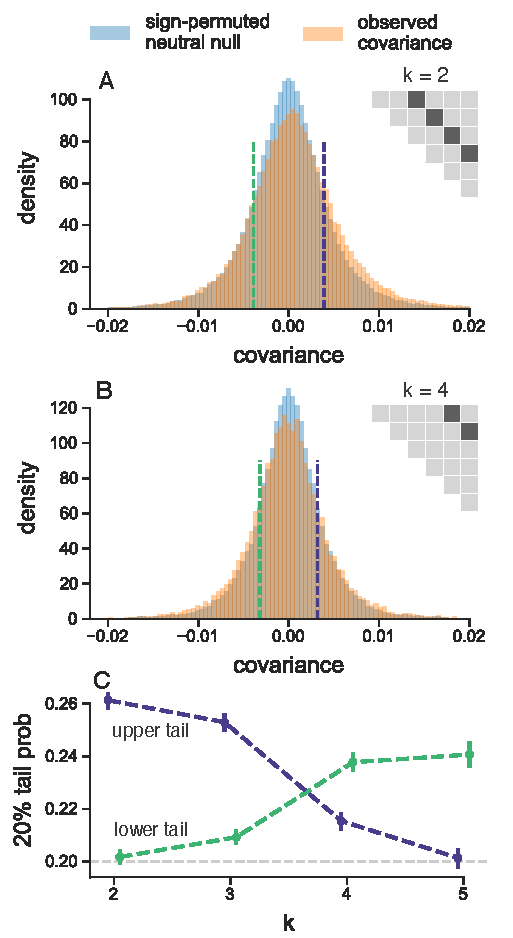
\includegraphics[]{figure-3-revision.pdf}

  \caption{\footnotesize {\bf A}, {\bf B}: The distribution of temporal
    covariances calculated in 100kb genomic windows from the
    \textcite{Barghi2019-qy} study, plotted alongside an empirical neutral null
    distribution created by recalculating the windowed covariances on 1,000
    sign permutations of allele frequency changes within tiles. The histogram
    bin number is 88, chosen by cross validation (Supplementary Materials
    \ref{suppfig:barghi-cross-validation-binsize}). In subfigure {\bf A},
    windowed covariances $\cov(\Delta p_t, \Delta p_{t+k})$ are separated by
    $k=2 \times 10$ generations and in subfigure {\bf A} the covariances are
    separated by $k=4 \times 10$ generations; each $k$ is an off-diagonal from
    the variance diagonal of the temporal covariance matrix (see cartoon of
    upper-triangle of covariance matrix in subfigures {\bf A} and {\bf B},
    where the first diagonal is the variance, and the dark gray indicates which
    off-diagonal of the covariance matrix is plotted in the histograms). {\bf
    C}: The lower and upper tail probabilities of the observed windowed
    covariances, at 20\% and 80\% quintiles of the empirical neutral null
    distribution, for varying time between allele frequency changes (i.e. which
    off-diagonal $k$). The confidence intervals are  $95\%$ block-bootstrap
  confidence intervals, and the light gray dashed line indicates the 20\% tail
probability expected under the neutral null. Similar figures for different
values of $k$ are in Supplementary Figures
\ref{suppfig:barghi-empnull-tilecovs}. }

    \label{fig:figure-3} 
\end{figure}


We observed that in the longest study  we analyzed \parencite{Barghi2019-qy},
some genome-wide temporal covariances become negative at future timepoints (see
the first two rows in Figure \ref{fig:figure-1}A). This shows that alleles that
were on average going up initially are later going down in frequency, i.e.
that the average direction of selection experienced by alleles has flipped.
This might reflect either a change in the environment or the genetic
background, due to epistatic relationships among alleles altered by frequency
changes (which can occur during an optima shift; \cite{Hayward2019-kt}) or
recombination breaking up selective alleles. Such reversals in selection
dynamics could be occurring at other timepoints but the signal of a change in
the direction of selection at particular loci may be washed out when we
calculate our genome-wide average temporal covariances.  To address this
limitation, we calculated the distribution of the temporal covariances over
100kb windowed covariances (Figure \ref{fig:figure-3} shows these distributions
pooling across all replicates; see Supplementary Figure
\ref{suppfig:barghi-offset-replicate-panels} for individuals replicates). The
covariance estimate of each genomic window will be noisy, due to sampling and
genetic drift, and the neutral distribution of the covariance is complicated
due to linkage disequilibria, which can occur over long physical distances in
E\&R and selection studies \parencite{Nuzhdin2013-gf,Baldwin-Brown2014-cl}.  To
address this, we have developed a permutation-based procedure that constructs
an empirical neutral null distribution by randomly flipping the sign of
the allele frequency changes in each genomic window (i.e. a single random sign
flip is applied to all loci in a window). This destroys the systematic
covariances created by linked selection and creates a sampling distribution of
the covariances spuriously created by neutral genetic drift while preserving
the complex dependencies between adjacent loci created by linkage
disequilibrium.  This empirical neutral null distribution is conservative in
the sense that the variances of the covariances are wider than expected under
drift alone, as selection not only creates covariance between time
intervals, but also inflates the magnitude of allele frequency change within a
time-interval.  We see (Figure \ref{fig:figure-3} A and B) that there are an
empirical excess of windows with positive covariances between close timepoints
compared to the null distribution (a heavier right tail), and that this then
shifts to an excess of windows with negative covariances between more distant
timepoints (a heavier left tail)

We quantified the degree to which the left and
right tails are inflated compared to the null distribution as a function of
time, and see excesses in both tails in Figure \ref{fig:figure-3}C. This
finding is also robust to sign-permuting allele frequency changes on a
chromosome-level, the longest extent that gametic linkage disequilibria can
extend (Supplementary Figure \ref{suppfig:barghi-tailprobs-seqid}). We see a
striking pattern that the windowed covariances not only decay towards zero, but
in fact become negative through time, consistent with many regions in the
genome having had a reversed fitness effect at later timepoints.

\begin{figure}[!htb]
  \centering
  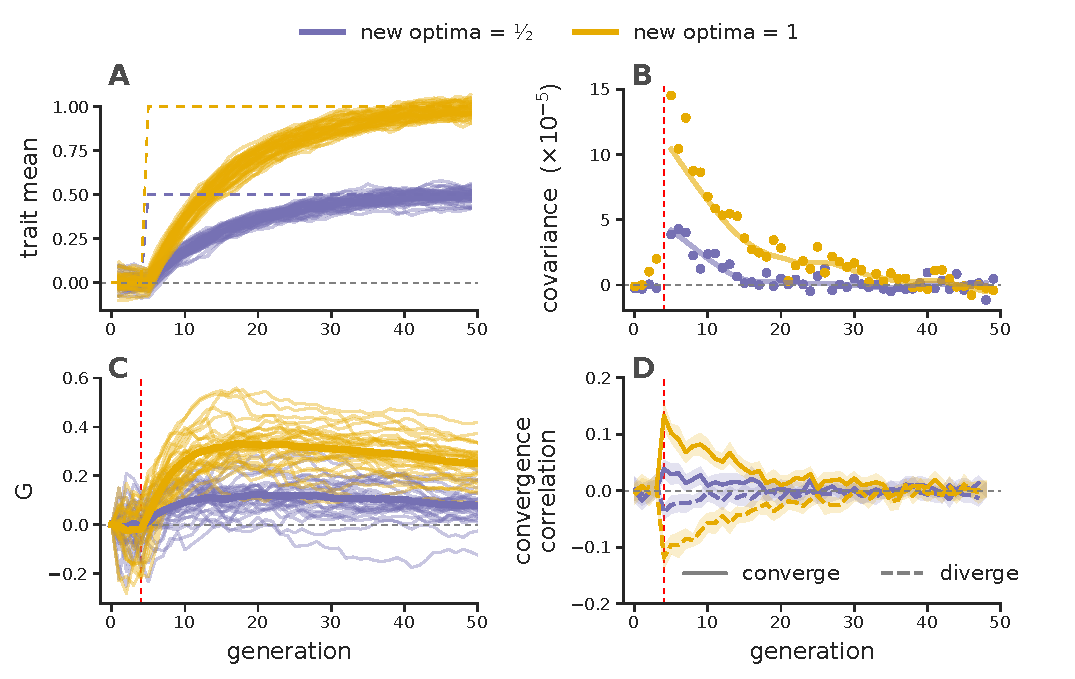
\includegraphics[width=\textwidth]{figure-4-edited.pdf}

  \caption{Forward-in-time simulations of demonstrate how temporal covariance,
    $G(t)$ trajectories, and convergence correlations arise during optima
    shifts of two different magnitudes, under Gaussian stabilizing selection.
    ({\bf A}) Trait means across 30 replicate before and after optima shifts (solid
    lines), for two different magnitudes (indicated by color). The optimal
    trait values are indicated by the purple and yellow dashed lines.  ({\bf B}) Mean
    temporal covariance $\cov(\Delta p_5, \Delta p_t)$ across 30 simulation
    replicates, where $t$ varies along the x-axis (points), with a
    loess-smoothed average (solid line). ({\bf C}) $G(t)$ trajectories through time,
    for 30 replicate simulations across two optima shifts. The solid line is a
    loess-smoothed average. ({\bf D}) The convergence correlations between two
    populations (each $1000$ diploids) split from a common population, that
    underwent either an optima shift in the same direction (converge) and
    opposite directions (diverge) at generation five. In subfigures ({\bf B}), ({\bf C}),
    and ({\bf D}), directional selection begins at generation five, when the optima
    shifts; this is indicated by the vertical dashed red line.}

  \label{fig:figure-4}
\end{figure}

Finally we used forward-in-time simulations to explore the conditions under
which temporal and convergent correlations arise. We show a subset of our
results for a model of stabilizing selection on a phenotype where directional
selection is induced by a sudden shift in the optimum phenotype of varying
magnitudes (Figure \ref{fig:figure-4}A). We find that positive temporal
covariances are produced by such selection (Figure \ref{fig:figure-4}B), and
that these positive temporal covariances can compound together to generate a
large proportion of allele frequency change being due to selection (i.e. large
$G(t)$) over the relatively short time periods similar to our analyzed
selection datasets span (Figure \ref{fig:figure-4}C).  The magnitude of
$G(t)$ increases with the strength of selection, i.e. the variance in
fitness, such that stronger selection generates larger proportions of allele
frequency change.  We find a similar picture of stronger convergent selection
pressures generating larger convergence correlations (Figure
\ref{fig:figure-4}D; see also Supplementary Materials Figure
\ref{suppfig:convergence-corrs} for how other factors impact convergence
correlations). 

These simulation results are often relatively insensitive to the number of loci
underlying the trait, suggesting that they are capturing highly polygenic
signals.  Indeed if only a small number of loci influence the trait, the $G(t)$
trajectories are typically much more stochastic across replicates (compare
Figure \ref{fig:figure-1}B to Supplementary Material Figure
\ref{suppfig:sim-expfit-Gs}). This again suggests that the genome-wide linked
selection response we see in the \textcite{Barghi2019-qy} data is highly
polygenic.  Using our simulations we find that sampling only every 10
generations does indeed mean that our estimates of $G(t)$ are an underestimate
of the contribution of linked selection as they cannot include the covariance
between closely spaced generations (see Supplementary Material Figure
\ref{suppfig:supp-blocks}).

Additionally, we explored other selection schemes. We find that the long term
dynamics of the covariances under directional truncation selection, which
generates substantial epistasis, are richer than we see under GSS and
multiplicative selection (Supplementary Material Figure
\ref{suppfig:supp-trunc}).  We also conducted simulations of purifying
selection alone (i.e. background selection) and find that this can also
generate positive temporal covariances (Supplementary Material Figure
\ref{suppfig:supp-bgs-covs}) and under some circumstances, can even generate
convergence correlations (Supplementary Material Figure
\ref{suppfig:supp-bgs-converg}). Thus it is unlikely that the signatures of
linked selection we see are entirely the result of the novel selection pressure
the populations are exposed to, and some of this selection may be ongoing
purifying selection. Only in the case of the Longshanks experiment, does the
control line allow us to conclude that selection that is due to the novel
selection pressure.

While none of our experiments have selected the populations in divergent
directions, in our simulations we find that such selection can generate
negative convergent correlations (Figure \ref{fig:figure-4}D). This suggests
that selection experiments combining multiple replicates, control lines, as
well as divergent selection pressures might be quite informative for unpacking
the contribution of particular selection pressures to genome-wide allele
frequency changes.

\section{Discussion}

Since the seminal analysis of \textcite{Maynard_Smith1974-zr} demonstrating
that linked neutral diversity is reduced as an advantageous polymorphism sweeps
to fixation, over four decades of theoretical and empirical research has
bettered our understanding of linked selection.  One under-used approach to
understand the genome-wide effects of selection on polygenic trait (e.g.  on
standing variation, stems from an early quantitative genetic model of linked
selection \parencite{Robertson1961-ho} and its later developments
(\cite{Santiago1995-hx,Santiago1998-bs,Wray1990-zf,Woolliams1993-qo}; see also
\cite{Barton2000-zg} for a comparison of these models with classic hitchhiking
models). Implicit in these models is that autocovariance between allele
frequency change is created when there is heritable fitness variation in the
population, a signal that may be readily detected from temporal genomic data
\parencite{Buffalo2019-io}.  Depending on how many loci affect fitness, even a
strong effect of linked selection may not be differentiable from genetic drift
using only single contemporary population samples or looking at temporal allele
frequency change at each locus in isolation. In this way, averaging summaries
of temporal data allows us to sidestep the key problem of detecting selection
from standing variation: that the genomic footprint leaves too soft of a
signature to differentiate from a background of genetic drift. In fact we find
that the temporal covariance signal is detectable even in the most extremely
difficult to detect soft sweep case: polygenic selection on highly polygenic
traits \parencite{Buffalo2019-io}.

It is worth building some intuition why temporal covariance allows us to detect
such faint signals of polygenic linked selection from temporal genomic data.
Each variant is subject to both variance in allele frequency due to drift and
sampling noise, which at any locus may swamp the temporal covariance signal and
creates spurious covariances. However, these spurious covariances do not share
a directional signal whereas the covariances created by linked selection do;
consequently, averaging across the entire genome, the temporal signal exceeds
sampling noise. 

Our analyses reveal that a sizable proportion of allele frequency change in
these populations is due to the (likely indirect) action of selection.
Capitalizing on replicated designs, we characterized the extent to which
convergent selection pressures lead to parallel changes in allele frequencies
across replicate populations, and found that a substantial proportion of
the response is shared across short timescales. These likely represent
substantial under-estimates of the contribution of linked selection because the
studies we have reanalyzed do not sequence the population each generation,
preventing us from including the effects of stronger correlations between
adjacent generations.  Furthermore, our estimation methods are intentionally
conservative, for example they exclude the contribution of selection that does
not persist across generations and selection that reverses sign; thus they can
be seen as a strong lower bound of the effects of selection, which we have
confirmed through forward-in-time simulations.

These estimates of the contribution of selection could be refined by using
patterns of linkage disequilibria (LD) and recombination which would allow
us to more fully parameterize a linked-selection model of temporal allele
frequency change \parencite{Buffalo2019-io}. The basic prediction is that
regions of higher linkage disequilibrium and lower recombination should have
greater temporal autocovariance than regions with lower LD and higher
recombination. However, one limitation of these pooled sequence datasets is
that none of the studies we reanalyzed estimated linkage disequilibria data for
the evolved populations.  While there are LD data for a natural population of
\emph{D. simulans} \parencite{Signor2018-wg,Howie2018-ay},  we did not find a
relationship between temporal covariance and LD.  We believe this is driven by
the idiosyncratic nature of LD in evolve-and-resequence populations, which
often extends over large genomic distances
\parencite{Nuzhdin2013-gf,Kelly2019-dc}. Future studies complete with LD data
and recombination maps would allow one to disentangle the influence of closely
linked sites from more distant sites in causing temporal autocovariance, and
allow the fitting of more parametric models to estimate population parameters
such as the additive genetic variance for fitness directly from temporal
genomic data alone \parencite{Buffalo2019-io}.

%very small effective population sizes, estimated
%at 300, 450, and 45 for the \textcite{Barghi2019-qy}, \textcite{Kelly2019-dc},
%and \textcite{Castro2019-uk} studies respectively

Our primary focus here has been on evolution in laboratory populations. It is
unclear whether we should expect a similar impact of selection in natural
populations. In some of these experiments, selection pressures may have been
stronger or more sustained than in natural populations
\parencite{Hendry1999-zu,Hairston2005-ga}. Conversely, these lab populations
were maintained at relatively small census sizes (Table
\ref{table:study_summary}), which will amplify the role of genetic drift,
and increase the frequency of rare deleterious alleles in selection lines
due to founder effects. The advantage of lab experiments is that they are
closed populations; in natural populations temporal covariance could also
arise from the systematic migration of alleles from differentiated populations.
Adapting these methods to natural populations will require either populations
that are reasonably closed to migration, or for the effect of migration to be
accounted for possibly either by knowledge of allele frequencies in source
populations or the identification of migrant individuals. 

While it challenging to apply temporal methods to natural populations there is
a lot of promise for these approaches
\parencite{Bergland2014-ij,Machado2018-cs}. Efforts to quantify the impact of
linked selection have found obligately sexual organisms have up to an 89\%
reduction in genome-wide diversity over long time periods
\parencite{McVicker2009-ax,Elyashiv2016-vt,Corbett-Detig2015-gt,Coop2016-gx,Comeron2014-nh}
Thus linked selection makes a sizeable contribution to long-term allele
frequency change in some species, and there is reason to be hopeful that we
could detect this from temporal data, which would help to resolve the
timescales that linked selection acts over in the wild. In our
reanalysis of the \textcite{Barghi2019-qy} study, we find evidence of complex
linked selection dynamics, with selection pressures flipping over time due to
either environmental change, the breakup of epistatic combinations or
advantageous haplotypes. Such patterns would be completely obscured in samples
from only contemporary populations. Thus, we can hope to have a much
richer picture of the impact of selection as temporal sequencing becomes more
common, allowing us to observe the effects of ecological dynamics in genomic
data \parencite{Hairston2005-ga}.

Furthermore, understanding the dynamics of linked selection over short
timescales will help to unite phenotypic studies of rapid adaptation with a
detectable genomic signature, to address long-standing questions concerning
linked selection, evolutionary quantitative genetics, and the overall impact
selection has on genetic variation. 

\section{Materials and Methods}

\subsection{Datasets Analyzed}

We used available genomic data data from four studies: pooled population
resequencing (pool-Seq) data from \textcite{Barghi2019-qy},
\textcite{Kelly2019-dc}, and \textcite{Bergland2014-ij}, and
individual-level sequencing data from \textcite{Castro2019-uk}. In all cases,
we used the variants kept after the filtering criteria of the original studies. 

\subsection{Variance and Covariance Estimates}

To remove systematic covariances in allele frequency change caused by tracking
the reference or minor allele, we randomly choose an allele to track
frequency for each locus. Then, we calculate the variance-covariance
matrix of allele frequency changes using a Python software package we have
written, available at \url{http://github.com/vsbuffalo/cvtk}. This
simultaneously calculates temporal variances and covariances, and replicate
covariances and uses the sampling depth and number of diploid individuals to
correct for bias in the variance estimates and a bias that occurs in covariance
estimates between adjacent timepoints due to shared sampling noise (see
Supplementary Material Sections \ref{supp:ind-depth-var-corr},
\ref{supp:cov-corr}, and \ref{supp:matrix-correction} for mathematical details
of these estimators). We assess that our bias correction procedure is working
adequately through a series of diagnostic plots that ensure that the procedure
removes the relationship between sampling depth and uncorrected variance and
covariances (Supplementary Figure \ref{suppfig:bergland-correction}).  Through
our simulations we find that our estimates can differ based on how fixations
and losses are handled in long time-series (Supplementary Material Section
\ref{supp:fixation}) but none of our findings in the main text are
qualitatively altered by this decision (Supplementary Material Figures
\ref{suppfig:supp-fig-1-nofix} and \ref{suppfig:supp-fig-3-nofix}).


\subsection{Estimating Uncertainty with a Block Bootstrap}

To infer the uncertainty of covariance, convergence correlation, and $G(t)$
estimates, we used a block bootstrap procedure. This bootstrap procedure
resamples blocks of loci, rather than individual loci, to infer the
uncertainty of a statistic in the presence of unknown correlation between loci.
As most estimators in this paper are ratios (e.g. covariance standardize by
sample heterozygosity, $G(t)$, and the convergence correlation), which we
estimate with a ratio of averages, we exploit the linearity of expectation for
efficient computation of bootstrap samples (see Supplementary Material Section
\ref{supp:block-bootstrap} for details).

\subsection{Partitioning Unique and Shared Selection Effects in the Longshanks Study}
\label{sec:mm-partition}

The unselected control line in the Longshanks experiment allows us to
additionally partition the total variance in allele frequency change into
drift, shared effects of selection, and unshared effects of selection between
selected replicates. We begin by decomposing the allele frequency change in
Longshanks line 1 (LS1) as $\Delta p_{t,\mathrm{LS1}} = \Delta_{_{D}}
p_{t,\mathrm{LS1}} + \Delta_{_{U}} p_{t,\mathrm{LS1}} + \Delta_{_S}
p_{t,\mathrm{LS}}$ where these terms are the drift in Longshanks replicate 1
($\Delta_{_D} p_{t,\mathrm{LS1}}$), selection unique to the LS1 replicate
($\Delta_{_U} p_{t,\mathrm{LS1}}$), and selection response shared between the
two Longshanks replicates ($\Delta_{_S} p_{t,\mathrm{LS}}$) respectively (and
similarly for the Longshanks line 2, LS2). By construction, this decomposition
assumes that each of these terms are uncorrelated within replicates, so the
contribution of each term to the total variance in allele frequency change,
$\var(\Delta p_{t,\mathrm{LS1}})$, is the variance of that term's allele
frequency change. 

We estimate the effects of selection by first calculating the fraction of the
total variance explained by drift. We assume the variance in allele frequency
change observed in the unselected control line ($\var(\Delta
p_{t,\mathrm{Ctrl}})$) is driven entirely by neutral genetic drift, and since
an identical breeding scheme was used across all three replicates (except
breeders for the control line were chosen at random), we can use this as an
estimate of the contribution of neutral genetic drift in the selected lines,
$\var(\Delta p_{t,\mathrm{Ctrl}}) = \var(\Delta_{_{D}} p_{t,\mathrm{LS1}}) =
\var(\Delta_{_{D}} p_{t,\mathrm{LS2}})$. Then, we can estimate the increase in
variance in allele frequency change due to selection as $(\var(\Delta
p_{t,\mathrm{LS1}}) + \var(\Delta p_{t,\mathrm{LS2}}))/2 - \var(\Delta
p_{t,\mathrm{Ctrl}})$ and the shared effect of selection across selected lines
as $\cov(\Delta p_{t,\mathrm{LS1}}, \Delta p_{t,\mathrm{LS2}})$. Finally, the
covariance in allele change between replicates is used to estimate the shared
effects of selection between lines, $\cov(\Delta p_{t,\mathrm{LS1}}, \Delta
p_{t,\mathrm{LS2}}) = \var(\Delta_{_S} p_{t,\mathrm{LS}})$.

\subsection{Windowed Covariance and the Empirical Neutral Null}

Throughout the paper, we use genomic windows for the block-bootstrap procedure.
For the \emph{D. simulans} and \emph{D.  melanogaster} data from the
\textcite{Barghi2019-qy}, \textcite{Kelly2019-dc}, and
\textcite{Bergland2014-ij} studies, we used large megabase windows for the
block bootstrap procedure, while we used a ten megabase window for the large
mouse genome data from the \textcite{Castro2019-uk} study. 

Given evidence of a reversal in the direction of selection at later timepoints
in the \textcite{Barghi2019-qy} study, we calculated windowed temporal
covariances on 10 kilobase windows and looked at the distribution of these
covariances through time. We compare these distributions of windowed
covariances to an empirical neutral null created by randomly permuting the sign
of allele frequency change at the block level (to preserve the correlation
structure between loci due to LD). This destroys the systematic covariances in
allele frequency change created by linked selection, which emulates a frequency
trajectory under drift. This approach is conservative, since heritable fitness
variation also inflates the magnitude of allele frequency change more than
expected under drift, but we do not change these magnitudes. Using this
empirical neutral null distribution of windowed covariances, we calculate how
much of the observed windowed covariance distribution falls outside of
empirical null distribution for different tail probabilities. While the
comparison between the distribution of 10 kilobase windowed covariances to the
empirical neutral null created from sign-permuting 10 kilobase windows is most
natural, we wanted to ensure that our finding that the shift from mostly
positive to mostly negative windowed covariances through time (Figure
\ref{fig:figure-3}) was robust to LD extending beyond the range of these 10
kilobase windows. We took the conservative approach of also sign-permuting at
the chromosome-level, and found the same qualitative shift (Supplementary
Figure \ref{suppfig:barghi-tailprobs-seqid}).

\subsection{Forward-in-time Simulations}

To explore how aspects of genetic architecture, model of selection, and
experimental design impact temporal covariance, the $G(t)$ trajectories, and
convergence correlations, we ran extensive forward-in-time using SLiM
\parencite{Haller2019-vu}; here we discuss the Gaussian Stabilizing Selection
simulations in Figured \ref{fig:figure-4}, but Supplementary Materials Section
\ref{supp:forward} describes these simulation routines in more detail as well
as additional simulations we have conducted.

We simulated directional selection on a trait by first burning in a population
of $N = 1000$ diploids under GSS for $10N$ generations with the stabilizing
selection trait variance $V_s = 1$ and an optima set at zero.  We note that the
small burnin population size means that these simulations should not be taken
as reflecting any specific natural population and they are for illustrative
purposes only.  We targeted a polygenic architecture by setting the trait
mutation rate to $10^{-8}$ per basepair, per generation, in addition to having
a separate neutral mutation of $10^{-8}$ which created neutral mutations which
we used to calculate the temporal covariances. Our simulated region was 50
megabases in length (about one quarter of a \emph{Drosophila} chromosome), and
trait alleles were randomly selected to have a $\pm 0.01$ effect size. By
tracking the trait mean through the burnin, we found it converged as expected.
After the burnin, the population was split into two different replicate
populations, to capture the effect of bottlenecks in selection experiments
(these population sizes varied between 50, 500, and 1000 diploids; the
later representing no bottleneck). Each population then underwent an optima
shift of either 0.1, 0.5, or 1 on generation five, with the first four
generations serving as a control. These optima shifts were either in the same
direction (converging), different directions (diverging), or only one optima
shifted (as a control). By tracking the trait mean, we saw that it converged as
expected during burnin, and had the appropriate response to selection
(Supplementary Material Figure \ref{suppfig:gss-zbar}). Using the neutral
population frequency data from these simulations, we calculated the temporal
covariances, $G(t)$ trajectories, and convergence correlations.


\section{Acknowledgments} 

We would like to thank the authors of the original studies we have analyzed,
including Neda Barghi, Nick Barton, Alan Bergland, Frank Chan, Kimberly Hughes,
John Kelly, Dmitri Petrov, Campbell Rolian, Christian Schl{\"o}tterer. We would
also like to thank Doc Edge for helpful statistical advice, and Dave Begun,
Erin Calfee, Sarah Friedman, Andy Kern, Chuck Langley, and Michael Turelli,
Matt Osmond, Peter Ralph, Sivan Yair for helpful discussions. Additionally, we
thank Guy Sella and an anonymous reviewer whose comments greatly improved the
manuscript. This research was supported by an NSF Graduate Research Fellowship
grant awarded to VB (1650042), and NIH (R01-GM108779) and NSF (1353380) awarded
to GC.

\printbibliography
\end{document}
